%!TEX root = ../thesis.tex
%*******************************************************************************
%****************************** Third Chapter **********************************
%*******************************************************************************
\chapter{Methodology and Results}\label{cha:4}

% **************************** Define Graphics Path **************************
\ifpdf
\graphicspath{{Chapter4/Figs/Raster/}{Chapter4/Figs/PDF/}{Chapter4/Figs/}}
\else
\graphicspath{{Chapter4/Figs/Vector/}{Chapter4/Figs/}}
\fi

Building on the theory from \Cref{cha:2}, this chapter details the practical application and validation of our framework.
\begin{enumerate}
  \item We first establish practical design guidelines from our theory and provide a specific instantiation of our framework for solving PDE-based forward and inverse problems.
  \item Next, we conduct preliminary tests on 1D Darcy flow to verify our method and gain practical insights.
  \item Finally, we present our main results, applying the framework to challenging 2D Darcy and Navier-Stokes equations.
\end{enumerate}

\section{Design Choices} \label{sec:dp}
Our theory provides three key design choices which we discuss below. These are the choice of noise, model capacity, and noise scale factor \(\gamma(t)\).

\subsection{Tradeoff between noise regularity and learnability} \label{sec:design1}
The choice of noise and model capacity are closely tied, so we discuss them together.  Our results on well-posedness require the noise to be sufficiently rough such that the target data (and also the source data in the case of inverse problems) to be supported on the Cameron-Martin space \(H_{C}\) (see Remark \ref{rem:hc}). Consequently, the networks \(\widetilde{\varphi}, \widetilde{\eta}\) must have enough capacity to process the less regular interpolant \(x_{t}\), and predict the rough training targets \(\dot{\alpha}(t)\xi_{0} + \dot{\beta}(t) \xi_{1}\) and \(z\).

However, excessively rough noise is detrimental for two reasons. First, it creates a more difficult learning problem, as the input \(x_{t}\) is also rougher and less informative, and the noise target \(z\) is harder for the denoiser \(\widetilde{\varphi}\) to predict. Second, it can harm sample quality: the Wasserstein-2 error bound in \Cref{eqn:w2} grows exponentially with the Lipschitz constant \(\widetilde{L}\) of the \textit{learned} approximations \(\widetilde{\varphi}, \widetilde{\eta}\). A rougher input \(x_{t}\) and noise target can lead to a larger \(\widetilde{L}\), weakening the performance guarantee.

This tension creates a practical ``sweet spot'' where noise must be just rough enough to satisfy the theoretical condition that \(\xi_{0}, \xi_{1}\) are supported in \(H_{C}\), but smooth enough to ensure a tractable learning problem and well-behaved Lipschitz constant. In this work, we employ implicit regularisation through our choice of network architecture and leave explicit control over network smoothness to future work.

\subsection{Choice of \(\gamma(t)\)}
As detailed in \Cref{sec:tc}, the noise scaling factor \(\gamma\) must be chosen such that \(\frac{1}{\gamma(t)}\) is integrable on \([0 ,1]\). In practice, this means
\begin{equation}
  \lim\limits_{t \to 0} \frac{t}{\gamma(t)} = \lim\limits_{t \to 1} \frac{1-t}{\gamma(t)} = 0,\label{eqn:integrability}
\end{equation}
that is, \(\gamma(t)\) must approach zero more slowly than \(t\) near the endpoint \(t=0\) (and similarly for \(1-t\) near \(t=1\)). Then, during sampling we solve the time-changed CB-SDE (\ref{eqn:tccbsde}) which re-parameterises the integration for numerical stability. % TODO: note this also helps for finite dimensional SI

% The interpolation schedule \(\alpha(t)\xi_{0} + \beta(t)\xi_{1}\) must also be chosen to encuorage learnability for the velocity and denoiser. Poorly chosen schedules can compromise learnability in two key ways. First, schedules which interpolate at a highly non-uniform rate can direct learning difficulty into a small window of time. This hinders training as the network is tasked to must learn complex dynamics with relatively few samples in that region. Second, if the signal component \(\alpha(t) \xi_{0} + \beta(t) \xi_{1}\) becomes too small relative to scaled noise \(\gamma(t)\), then the interpolant \(x_{t}\) becomes less informative for the velocity and more informative for the denoiser. This can worsen the approximation error for the overall drift, especially during intermmediate time steps where the weighted coefficient \(\hat{c}(t)\) on the denoiser is small. A well-designed schedule must therefore ensure a gradual and predictable evolution from source to target.

% : a well-chosen schedule ensures the prediction task remains tractable across the entire time interval. Following the literature in rectified flow \citep{liu2022flow}, the canonical choice is a linear interpolation schedule: \(\alpha(t) \coloneqq 1-t, \beta(t) \coloneqq t\), which corresponds to a straight path between \(\xi_0\) and \(\xi_1\) at a constant speed.
\section{Instantiation of Framework}
We now provide a concrete setup of the framework and algorithms that we use to solve PDE-based forward and inverse problems.

\subsection{Hilbert spaces} \label{sec:hs}
Throughout, we work with data that lie in the Hilbert space of square-integrable functions on a compact Euclidean subset: this will be \(L^{2} = L^{2}(D)\) where \(D = [0, 1]\) for functions defined on a unit interval \(D = [0, 1]^{2}\) for functions on the unit square. We equip this with the canonical \(L^{2}\)-inner product:
\[
  \ev{f, g}_{L^{2}} \coloneqq \int_{D} f(x) g(x) \dd{x}.
\]

We work with two distinct settings for source and target data. In the first, we address homogeneous data where \(\xi_{0}\) and \(\xi_{1}\) represent similar physical quantities and can be naturally modelled on the same function space. We therefore define the interpolant space as  \(H \coloneqq L^{2}\). This approach is suitable for problems like predicting a future fluid pressure field \(\xi_{1}\) from a past one \(\xi_{0}\).

In the second setting, we address heterogeneous data, where \(\xi_{0}\) and \(\xi_{1}\) are different physical quantities (e.g. a permeability field and a pressure field). Interpolating directly between these in a single channel would be unnatural and impose a difficult disentanglement task during learning. To provide a stronger inductive bias, we define the interpolant space as the \textit{product space} \(H \coloneqq L^{2} \times L^{2}\). Here, for a pair of source and target data functions, we simply define the data as \(\xi_{0} = (\xi_{0}', 0)\) and \(\xi_{1} = (0, \xi_{1}')\), where \(0\) represents the zero function on \(D\) and \(\xi_{0}', \xi_{1}' \in L^{2}\). Under this construction,  there is no signal bleed in the interpolant \(x_{t}\)  as heterogeneous data channels are kept separate. Note that more generally, the underlying data \(\xi_{0}', \xi_{1}'\) could reside in different Hilbert spaces. Since the product space \(H\) is still a Hilbert space, all results of our theory hold true for the new source and target random variables \(\xi_{0}'\) and \(\xi_{1}'\).

\subsection{Noise}
When \(H = L^{2}\), we define noise \(z\) as samples from a Gaussian process \citep{williams2006gaussian} with zero mean and radial basis function (RBF) kernel \(k\):
\[
  z \sim \mathrm{GP}(0, k), \text{ where } k(x, y) \coloneqq \exp(-\frac{1}{2\ell} \norm{x - y}^{2}_{D}).
\] equal to a radial basis function of gain \(1\) and varying length scales \(\ell > 0\) to investigate the impact of noise roughness on evaluation performance. This is equivalent to sampling \(z\) from a Gaussian measure \(N(0, C)\) on \(H\) where the covariance operator is trace-class and given by
\[
  Cf(x) \coloneqq \int_{D} f(y) k(x, y) \dd{y}.
\]

In the product space setting where \(H = L^{2} \times L^{2}\), we define the noise \(z\) as a pair of independent samples from this process, i.e. \(z = (z_{0}, z_{1})\) where each component \(z_{0}, z_{1} \overset{\text{i.i.d.}}{\sim} \mathrm{GP}(0, k)\). Formally, this is equivalent to sampling from a GP with matrix-valued kernel \(K\):
\[
  z \sim \mathrm{GP}(0, K), \text{ where } K(x, y) \coloneqq \mqty[k(x,y) & 0 \\ 0 & k(x,y)].
\]
Henceforth, we continue to use notation pertaining to the homogeneous data setting, but all statements are equally valid for heterogeneous data.

\subsection{Choice of \(\gamma(t)\)} Following \citep{albergo2023stochasticinterpolantsunifyingframework}, we define
\[
  \gamma(t) \coloneqq \sqrt{bt(1-t)}.
\]
This satisfies \Cref{eqn:integrability}, so \(\frac{1}{\gamma(t)}\) is integrable on \([0, 1]\). The following result provides necessary and sufficient conditions on the time change function \(\theta\) such that the time-changed coefficient \(\hat{c}(t) = c(\theta(t)) \dot{\theta}(t)\) (Equation \ref{eqn:chat}) on the denoiser is finite on \([0, 1]\). We provide the proof in \Cref{prf:lem:thetaconditions} in Appendix \ref{app:A}.

\begin{theorembox}
  \begin{restatable}{lemma}{restatelemthetaconditions}\label{lem:thetaconditions}
    A strictly increasing, bijective, continuously differentiable time change function \(\theta(t)\) on \([0, 1]\) is a valid change-of-time ensuring that \(\hat{c}(t)\) is finite on \([0, 1]\) if and only if \(\theta(t)\) satisfies the following conditions.
    \begin{enumerate}
      \item\label{lem:thetaconditions:1} \(\lim\limits_{t \to 1^{-}} \frac{\dot{\theta}(t)}{2(1-t)} < \infty \); and
      \item\label{lem:thetaconditions:2} \(\lim\limits_{t \to 0^{+}} \frac{\dot{\theta}(t)}{2t} < \infty \) if \(\varepsilon \neq \frac{b}{2}\).
    \end{enumerate}
  \end{restatable}
\end{theorembox}
\begin{remarkbox}
  \begin{remark}
    Intuitively, these conditions (\ref{lem:thetaconditions:1}) and (\ref{lem:thetaconditions:2}) mean that the \textit{rate of time change} decays to zero at the endpoints. This controlled deceleration is precisely what resolves the singularity.
  \end{remark}
\end{remarkbox}
For SDE inference, we will choose \(\varepsilon = \frac{b}{2}\), which simplifies the original coefficient to \(c(t) = -\sqrt{\frac{bt}{1-t}}\). This resolves the singularity at \(t=0\) leaving only the singularity at  \(t=1\) to be  managed by the time change. Therefore, only condition (\ref{lem:thetaconditions:1}) is required to ensure the time-changed coefficient \(\hat{c}(t)\) is finite on \([0, 1]\).

\subsection{Choice of \(\alpha(t)\) and \(\beta(t)\)}
Following work on rectified flow \citep{liu2022flow}, we choose \(\alpha(t)  \coloneqq 1-t\) and \(\beta(t) \coloneqq t\), which makes the signal \(\alpha(t) \xi_{0} + \beta(t) \xi_{1}\) a linear interpolation between source and target data. This straight line path has two advantages:
\begin{enumerate}
  \item The instantaneous velocity is \(\varphi(t, x_{t}) = \mathop{\mathbb{E}}\qty[\xi_{1} - \xi_{0} \mid \xi_{0}, x_{t}]\), which simplifies the training task as the network \(\widetilde{\varphi}\) targets the constant vector \(\xi_{1} - \xi_{0}\).
  \item The lack of curvature in the trajectory means that the ODE component is easier to solve during inference. In fact, in the deterministic case where \(\varepsilon = 0\), the probability flow ODE can be solved in just one step.
\end{enumerate}

\subsection{Training and sampling algorithms}
We provide concrete details we use for training and sampling in \Cref{alg:training,alg:sampling}. During training, times \(t\) are sampled uniformly on \([0, 1]\). During sampling, we solve the time-changed CB-SDE (\ref{eqn:tccbsde}) using an arbitrary SDE solver (or ODE solver if \(\varepsilon = 0\)) with update function \texttt{OneStep}. On a computer, functions must be discretised, so we introduce a grid \(\mathcal{G} = \{s^{(j)}\}_{j=1}^{J}\) of sensor locations, where each sensor \(s^{(j)}\) is an input point on the domain \(D\). In calculating the losses, the squared \(H\)-norm becomes a summation over the sensors, leading to standard mean-squared error loss.

\begin{figure}
  \begin{singlespace}
    \begin{algorithm}[H]
      \caption{Training}\label{alg:training}
      \begin{algorithmic}[1]%
        \Require Paired training data \(\mathcal{D} \coloneqq \{(\xi_{0}^{(i)}, \xi_{1}^{(i)})\}_{i=1}^{I}\), where each training example \((\xi_{0}^{(i)}, \xi_{1}^{(i)}) \sim \mu\)
        \Require Batch size \(B\)
        \Require Discretisation grid \(\mathcal{G} \coloneqq \{s^{(j)}\}_{j=1}^{J}\) of sensor locations, where each sensor  \(s^{(j)} \in D\)
        \State Initialise networks \(\widetilde{\varphi}, \widetilde{\eta}\)
        \While{loss not low enough}
        \State Sample \(\{z^{(i)}\}_{i=1}^{B}\) evaluated at points in \(\mathcal{G}\), where each \(z^{(i)} \overset{\text{i.i.d.}}{\sim} \operatorname{GP}(0, k)\)
        \State Subsample a batch \(\{(\xi_{0}^{(i)}, \xi_{1}^{(i)})\}_{i=1}^{B}\) from \(\mathcal{D}\) and evaluate at discretisation \(\mathcal{G}\)
        \State Sample times \(\{t^{(i)}\}_{i=1}^{B}\) where each \(t^{(i)} \overset{\text{i.i.d.}}{\sim} \operatorname{U}([0, 1])\)
        \State Let interpolant \(x_{t}^{(i)} \leftarrow \alpha(t^{(i)}) \xi_{0}^{(i)} +\beta(t^{(i)})\xi_{1}^{(i)} + \gamma(t^{(i)}) z^{(i)}\)
        \State Let loss \(\mathcal{L}(\widetilde{\varphi}) \leftarrow \frac{1}{B}\sum_{i=1}^{B}\frac{1}{J} \sum_{j=1}^{J} \qty(\big[\widetilde{\varphi}(t^{(i)}, x^{(i)}_{t}) - \big(\dot{\alpha}(t^{(i)}) \xi_{0}^{(i)} + \dot{\beta}(t^{(i)}) \xi_{1}^{(i)}\big)\big](s^{(j)}))^{2} \)
        \State Let loss \(
          \mathcal{L}(\widetilde{\eta}) \leftarrow \frac{1}{B} \sum_{i=1}^{B} \frac{1}{J}\sum_{j=1}^{J} \qty(\big[\widetilde{\eta}(t^{(i)}, x_{t}^{(i)}) - z^{(i)}\big](s^{(j)}))^{2},
        \)
        \State Perform gradient step on \(\mathcal{L}(\widetilde{\varphi})\) and \(\mathcal{L}(\widetilde{\eta})\).
        \EndWhile
      \end{algorithmic}
    \end{algorithm}

    \begin{algorithm}[H]
      \setlength{\abovedisplayskip}{2pt}
      \setlength{\belowdisplayskip}{2pt}
      \caption{Sampling}
      \label{alg:sampling}
      \begin{algorithmic}[1]
        \Require Test dataset \(\mathcal{T} \coloneqq \{\xi_{0}^{(i)}\}_{i=1}^{I}\)
        \Require Number of time steps \(T \geq 1\)
        \Require Trained networks \(\widetilde{\varphi}, \widetilde{\eta}\)
        \Require \(\varepsilon \geq 0\)
        \Require Time change function \(\theta\)
        \Require Any SDE (or ODE if \(\varepsilon = 0\)) solver with update function \texttt{OneStep}
        \State Construct time-changed approximate drift \[\hat{\widetilde{f}}(t, x_{0}, x) \leftarrow \widetilde{\varphi}(\theta(t), x_{0}, x)\dot{\theta}(t) + \qty(\dot{\gamma}(\theta(t)) - \frac{\varepsilon}{\gamma(\theta(t))}) \widetilde{\eta}(\theta(t), x_{0}, x)\dot{\theta}(t)\]
        \State Let \(\Delta t \leftarrow \frac{1}{T}\)
        \ForAll{\(i = 1, \ldots, I\)}
        \State Let \(X_{0}^{(i)} \leftarrow \xi_{0}^{(i)}\)
        \State Let \(t \leftarrow 0\)
        \While{ \(t \neq 1\) }
        \State Let \(X_{t + \Delta t}^{(i)} \leftarrow \texttt{OneStep}(t, \xi_{0}^{(i)}, X_{t}^{(i)}, \hat{\widetilde{f}}, \varepsilon, C, \Delta t)\)
        \State Update \(t \leftarrow t + \Delta t\)
        \EndWhile
        \EndFor
      \end{algorithmic}
      \Return \(\{X_{1}^{(i)}\}_{i=1}^{I}\)
    \end{algorithm}
  \end{singlespace}
\end{figure}

The algorithms are stated for the forward problem, i.e. bridging from source \(\xi_{0} \sim \mu_{0}\) to conditional target \(\mu_{1 \mid 0}(\dd{\xi_{1}, \xi_{0}})\), but analogous results for the reverse problem are given by considering approximations \(\widetilde{\varphi}^{\text{rev}}, \widetilde{\eta}^{\text{rev}}\) as in \Cref{sec:backwards} and initialising \(X_{0}^{(i)} \leftarrow \xi_{1}^{(i)}\) during sampling (note that the process is also solved forward in time).

An alternative method of discretisation is to consider projections of the data functions and noise onto an orthonormal basis of \(H\). If using eigenvectors of the covariance operator \(C\), then by the Karhunen-Loève theorem \citep{stark1986probability}, one can model the noise as independent zero-mean Gaussians with variances equal to the corresponding eigenvalue. In this case, mean-square error corresponds to taking the \(H\)-norm. This is akin to \citet{phillips2022spectral}, who consider diffusion models in the spectral domain.  However we do not take this approach, since our neural operator architectures are already designed to learn their own spectral representation via internal spectral convolution layers. Pre-projecting the data onto a fixed basis imposes an unnecessary bottleneck, prevent the network from learning the most effective representation. A direct sensor-based approach also avoids solving a costly eigenvalue problem.

We now turn to applications of this instantiation of our SI framework.

\section{Experimental Insights: 1D Darcy Flow} \label{sec:prelim}
We first conduct a series of preliminary experiments on a small dataset of functions defined on a line, that is, \(D = [0, 1]\) and use lightweight Fourier nerual operator (FNO; \citealp{li2020fourier}) networks for \(\widetilde{\varphi}\) and \(\widetilde{\eta}\). These experiments are less computationally expensive and designed to provide key insights for the more complex problems addressed in \Cref{sec:darcy2}.

Specifically, we aim to answer the following questions:
\begin{enumerate}
  \item How important does the noise smoothness affect model performance?
  \item What is the effect of different choices of time change functions \(\theta\)?
  \item Is there a benefit to sampling time \(t\) non-uniformly on \([0, 1]\) and according to the importance proscribed by the time change?
\end{enumerate}
\subsection{Experimental Setup}
\paragraph{Dataset}
We follow \citep{bahmani2025resolution} and consider a non-linear variant of Darcy's equation in 1D \citep{whitaker1986flow}:
\begin{equation}
  \dv{w}\qty[-\qty(0.2 + \psi^{2}(w)) \dv{\psi(w)}{w}] = u(w), \qquad w \in [0, 1], \psi(0) = \psi(1) = 0,\label{eqn:d1d}
\end{equation}
where \(u \sim \operatorname{GP}\) with RBF kernel and length scale \(0.05\) is a \textit{forcing function} and the solution \(\psi \in L^{2}\) is \textit{pressure}. Intuitively,  \(u(w)\) describes the environmental factors of fluid inflow/outflow at distances \(w \in [0, 1]\) along a unit-length pipe, and \(\psi(w)\) is the corresponding pressure along this pipe at \(w\). The quantity \(0.2 + \psi^{2}(w)\) is a pressure-dependent permeability.

The forward problem is as follows: given a specific forcing function \(u\), we aim to predict the (unique) corresponding pressure solution \(\psi\). Similarly, for the inverse problem, we are given a pressure solution \(\psi\) and aim to predict the forcing function \(u\) which produced that solution.

Using the same code provided by \citep{bahmani2025resolution}, we sample many forcing functions \(u\) and solve \Cref{eqn:d1d} using the finite element method to create a dataset of paired data with an 8000/1000/1000 train/dev/eval split. We discretise functions on 128 evenly-spaced points on the unit interval \([0, 1]\). We evaluate the accuracy of predictions using the relative \(L^{2}\)-error: for a prediction \(\widetilde{y} \in L^{2}\) and ground truth \(y \in L^{2}\), the relative \(L^{2}\)-error is given by
\[
  \frac{\norm{ \widetilde{y} - y}_{L^{2}}}{\norm{y}_{L^{2}}}.
\]
Computationally, we calculate these norms using Riemann summation over the 128 evenly spaced gridpoints on \([0, 1]\).

\paragraph{Architecture and hyperparameters}
We train \(\widetilde{\varphi}\) and \(\widetilde{\eta}\) as separate FNO networks with identical hyperparameters. Full details of the hyperparameters we use are given in \Cref{tbl:hyp1} in \Cref{app:B}. Since the source and target functions in our dataset exhibit a high degree of smoothness we follow our design guidance in \Cref{sec:design1} and use the following architectural choices to implicitly regularise the network, biasing towards smoother outputs:
\begin{enumerate}
  \item We restrict the number of Fourier nodes to \(16\), which discourages the networks from learning high-frequency components
  \item We apply separable convolutions, in which distinct depthwise convolutions are performed for each input channel, followed by a pointwise convolution across channels, to decouple spatial filtering and channel mixing, which lowers capacity in each convolution layer
\end{enumerate}

Since the forcing function \(u\) and pressure \(\psi\) describe distinct physical phenomena, we employ the product space form for our interpolants (\(H = L^{2} \times L^{2}\)), as detailed in \Cref{sec:hs}: for each pair \((u, \psi)\), we define the source to be \(\xi_{0} = (u, 0)\) and the corresponding target \(\xi_{1} = (0, \psi)\).

\subsection{Results and Insights}
\paragraph{Roughness of noise}
We first investigate the impact of noise roughness on model performance, by varying the length scale \(\ell\) of the RBF varies for the Gaussian process noise \(z)\). Throughout these experiments, we fix the time-change function \(\theta(t) \coloneqq 2t -t^{2}\), which we call \texttt{ease-out}, and sample for \(T=100\) time steps.

\begin{figure}
\centering
\begin{subfigure}[t]{0.45\linewidth}
  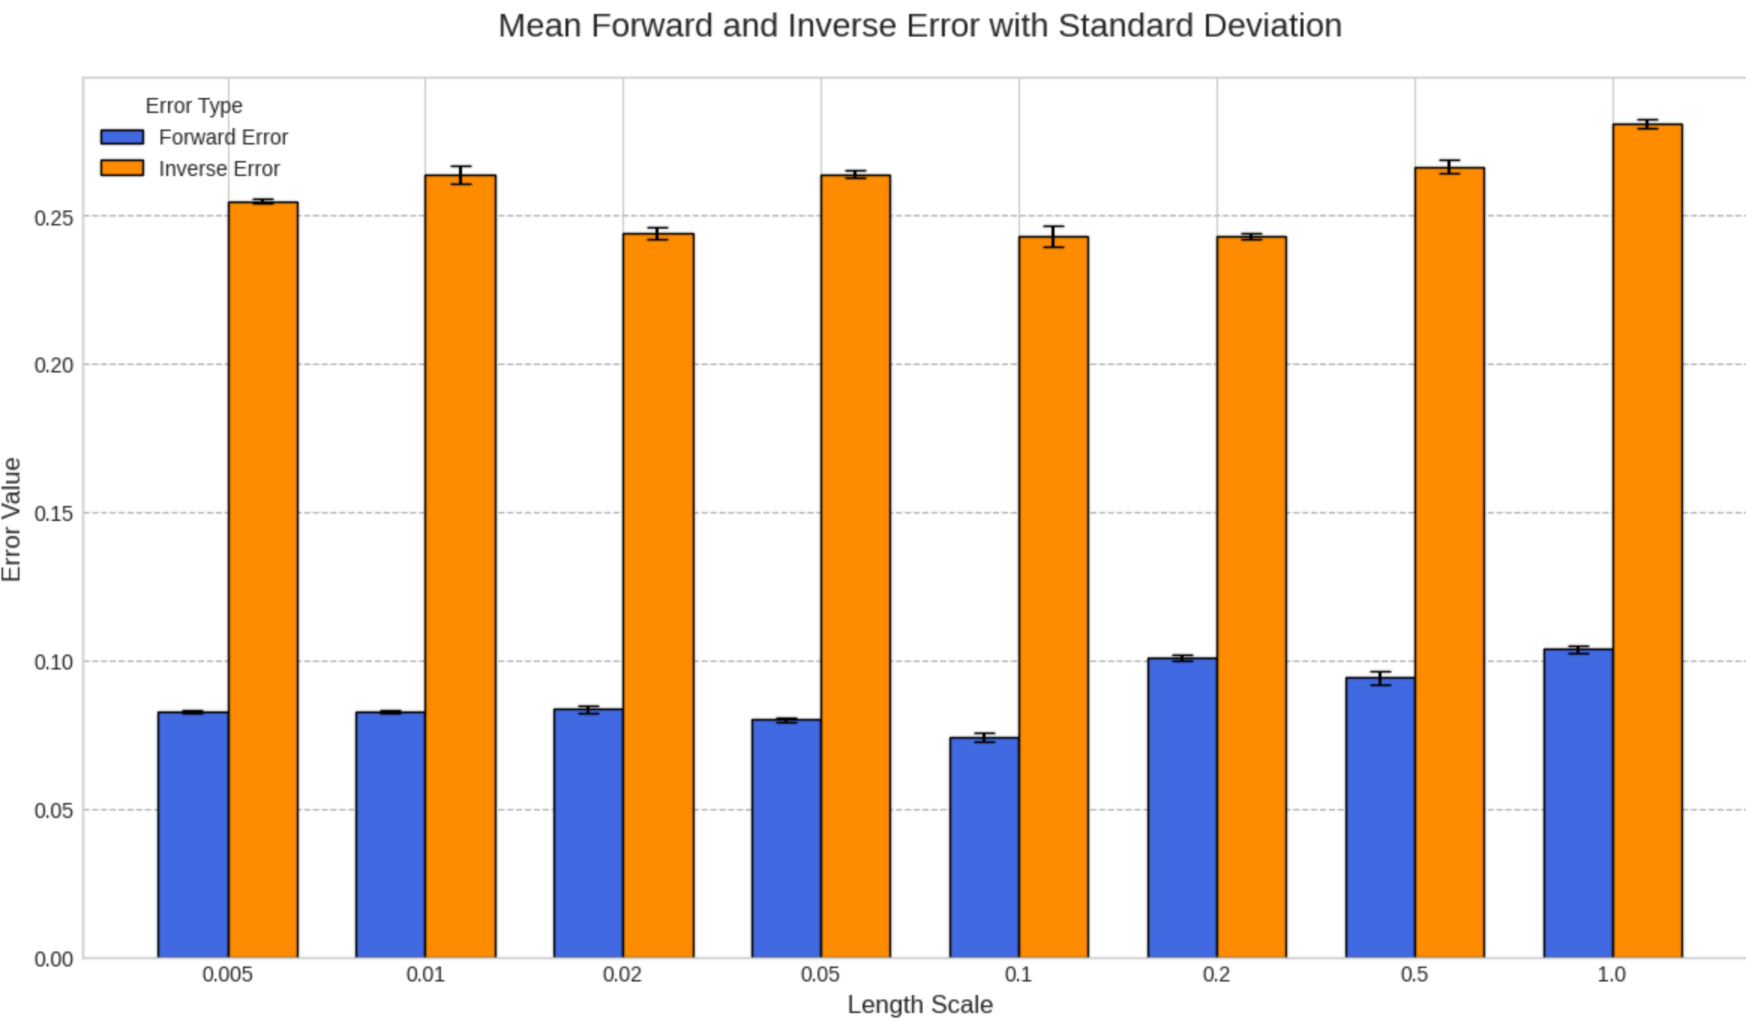
\includegraphics[width=\linewidth]{len_darcy_1d.png}
  \caption{Relative \(L^{2}\)-error of forward and inverse tasks for the 1D Darcy flow problem as the length scale  varies for the Gaussian process noise. Means and standard deviations are plotted across three inference runs.}\label{fig:d1dlen}
\end{subfigure}%
\hfill%
\begin{subfigure}[t]{0.45\linewidth}
  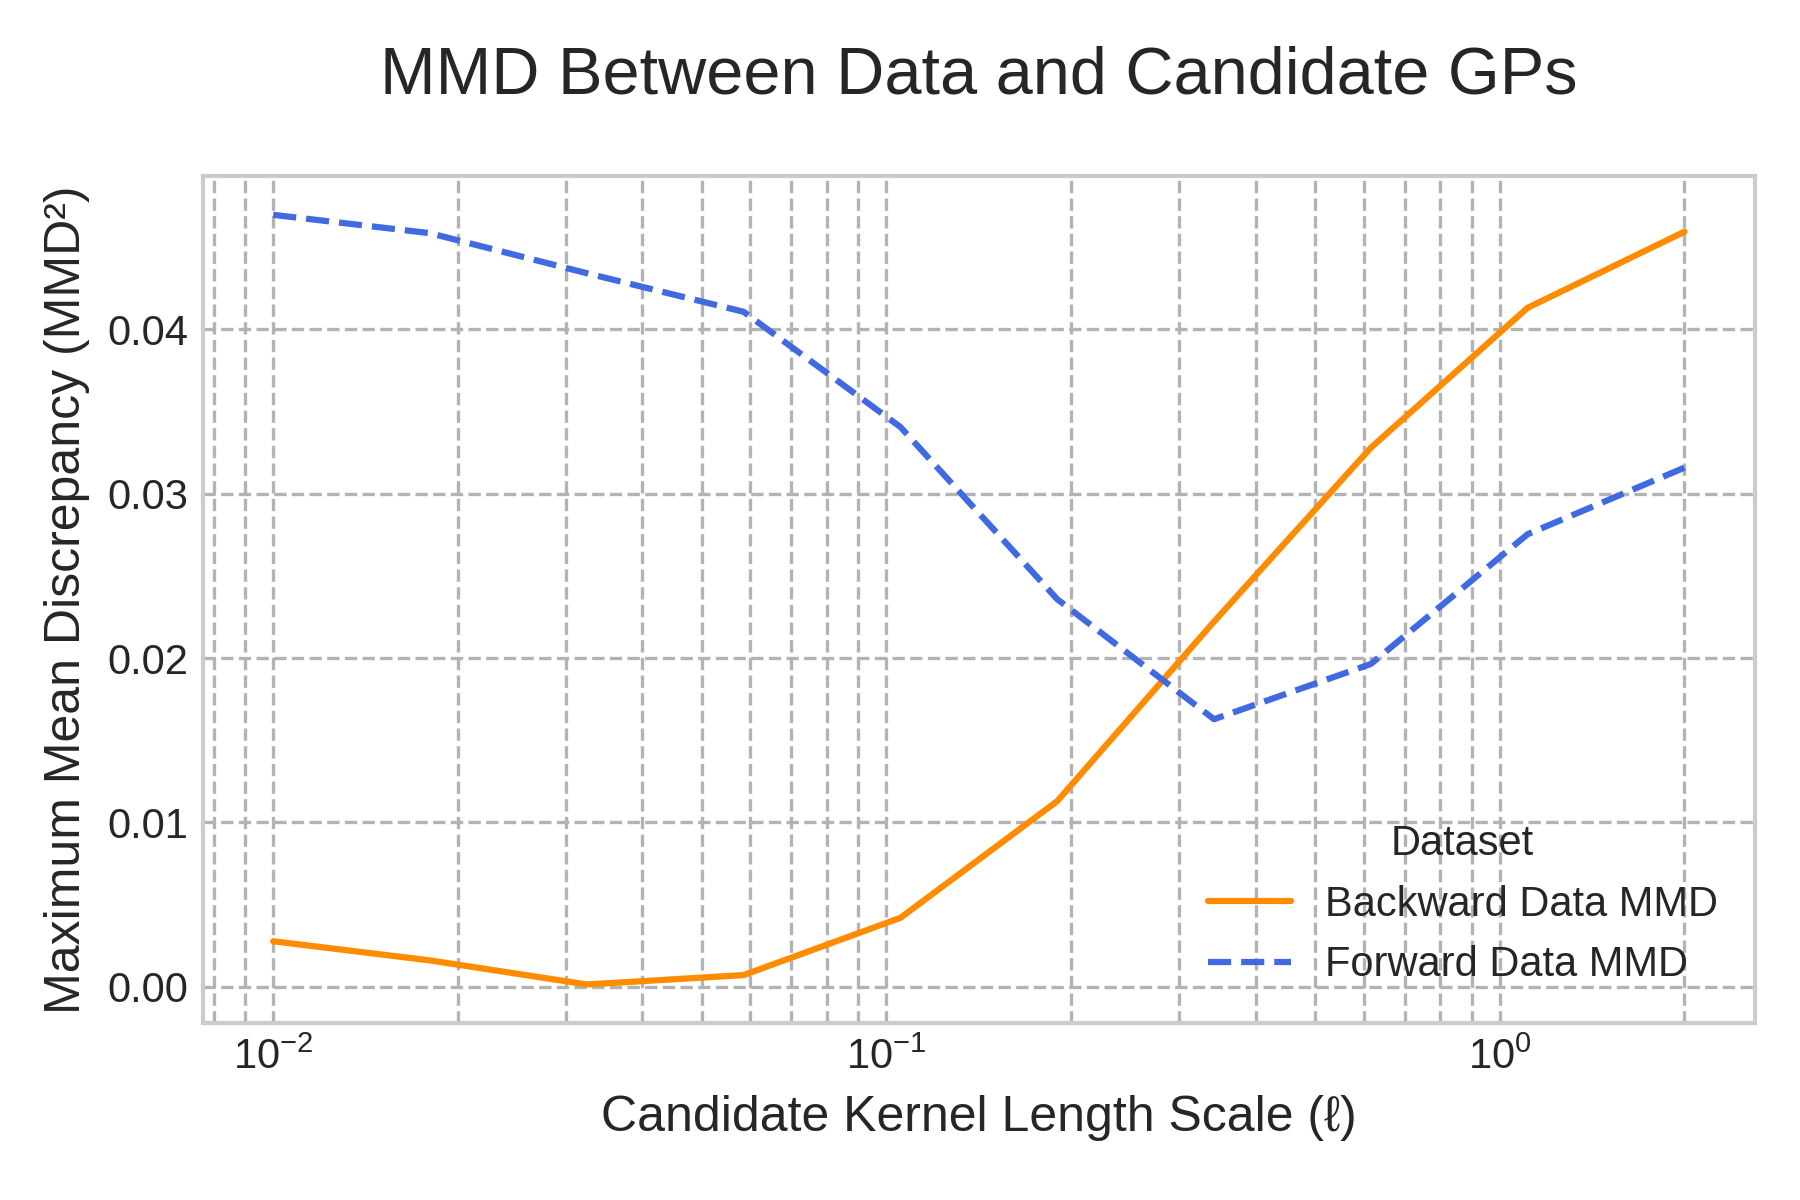
\includegraphics[width=\linewidth]{mmd_darcy_1d.png}
  \caption{Estimated maximum mean discrepency between forcing functions (backward data) and pressure functions (forward data) for different candidate RBF kernel length scales.}\label{fig:d1dmmd}
\end{subfigure}
\caption{}
\end{figure}

\Cref{fig:d1dlen} shows that the optimal noise regularity is task-dependent: the optimal performance is achieved at  \(\ell = 0.2\) for the inverse task and \(\ell = 0.05\) for the forward task.

To gain a sense of the characteristic smoothness of target data for the forward and inverse tasks, we \Cref{fig:d1dmmd} shows the estimated maximum mean discrepency (MMD; \citealp{gretton2012kernel}) between samples of Gaussian processes with varying length scales and the functions \(u\) and \(\psi\) across the training dataset. As expected, the minimum MMD for backward data (\(u\)) is attained close  \(0.05\), which is the ground truth since \(u\) are exact samples from a GP with length scale \(0.05\). The MMD for forward data (\(\psi\)) is lowest at around \(0.3\), reflecting the fact that the pressure field is a smoother physical quantity.

\Cref{fig:d1dlen} confirms the hypothesis of a ``sweet spot'' length scale, however the location of this sweet spot varies between tasks. For both tasks, there is a noticeable dip in performance when the length scale is matched most closely between the noise and the target. We believe this is because when matched, the prediction tasks are more difficult since the noise and signal components of the interpolant \(x_{t}\) are more difficult to distinguish between. Peak performance in both tasks happens at the length scale increment just before the target is matched. Hence, we conclude from these experiments that \textit{noise should be made just rougher than the data, so it easy to distinguish between signal and noise components in the intrepolant, but not too rough so as to degrade performance}.

Since \Cref{fig:d1dmmd} shows that the characteristic smoothness in source and target data differ by almost an order of magnitude, we run an additional experiment in which the length scales of noise are different across the channels, corresponding to their best performance in \Cref{fig:d1dlen}: we set the \(u\)-channel to have length scale \(\ell=0.02\) and the \(\psi\)-channel to have length scale \(\ell=0.1\). This model with heterogeneous noise scales performs best, achieving relative \(L^{2}\) errors of \(6.9_{\pm 0.1}\%\) and \(19.9_{\pm0.2}\%\) respectively. For the remainder of this section, we use this choice of heterogeneous noise.

\paragraph{Time change function}

We now investigate the effect of the time change function \(\theta\) on model performance. We consider the six schedules defined in \Cref{fig:schedules}. All schedules except for \texttt{ease-in} and \texttt{ease-in-*} satisfy condition (\ref{lem:thetaconditions:1}) of \Cref{lem:thetaconditions}, and \texttt{ease-in-out} and \texttt{ease-in-out-*} additionally satisfy condition (\ref{lem:thetaconditions:2}).

\begin{figure}[tbhp]
\centering
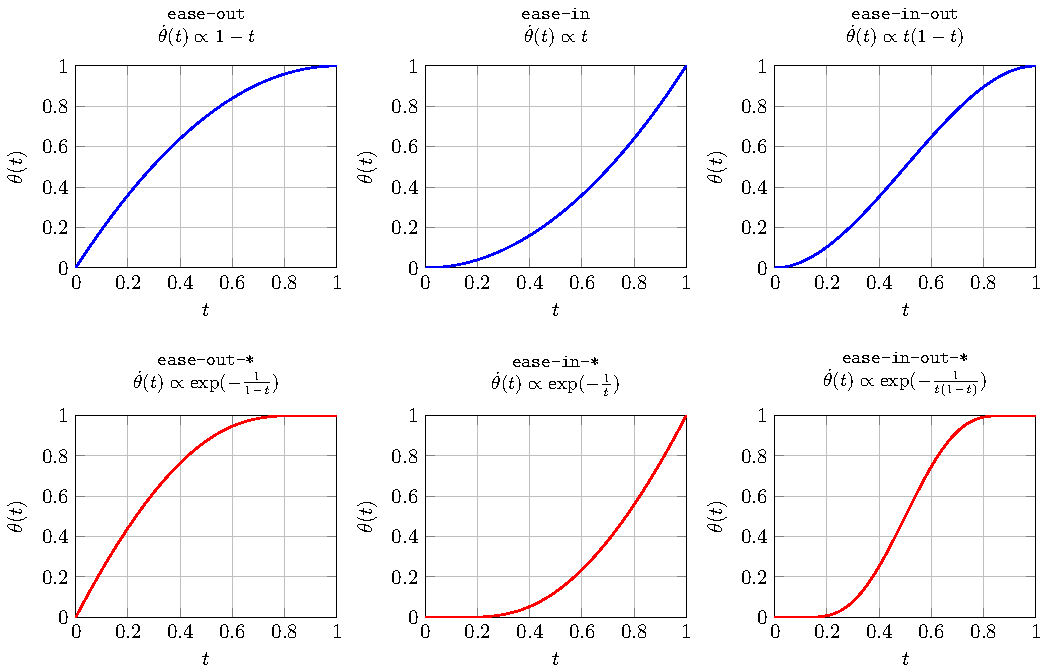
\includegraphics[width=\linewidth]{schedules.pdf}
\caption{We define six time schedules via their derivatives, omitting a normalising constant which ensures \(\theta(0) = 0, \theta(1)=1\). }\label{fig:schedules}
\end{figure}

\Cref{fig:schedulesr} presents our results and highlights that  time-change schedule is critical for ensuring numerical stability during sampling. The schedules that are not well-behaved at the starting time \(t=0\), namely \texttt{ease-in}, \texttt{ease-in-*} and the baseline with no time change, exhibit errors orders of magnitude larger than the others. This empirically validates our theoretical stability conditions presented in \Cref{lem:thetaconditions}.

\begin{figure}[tbhp]
\centering
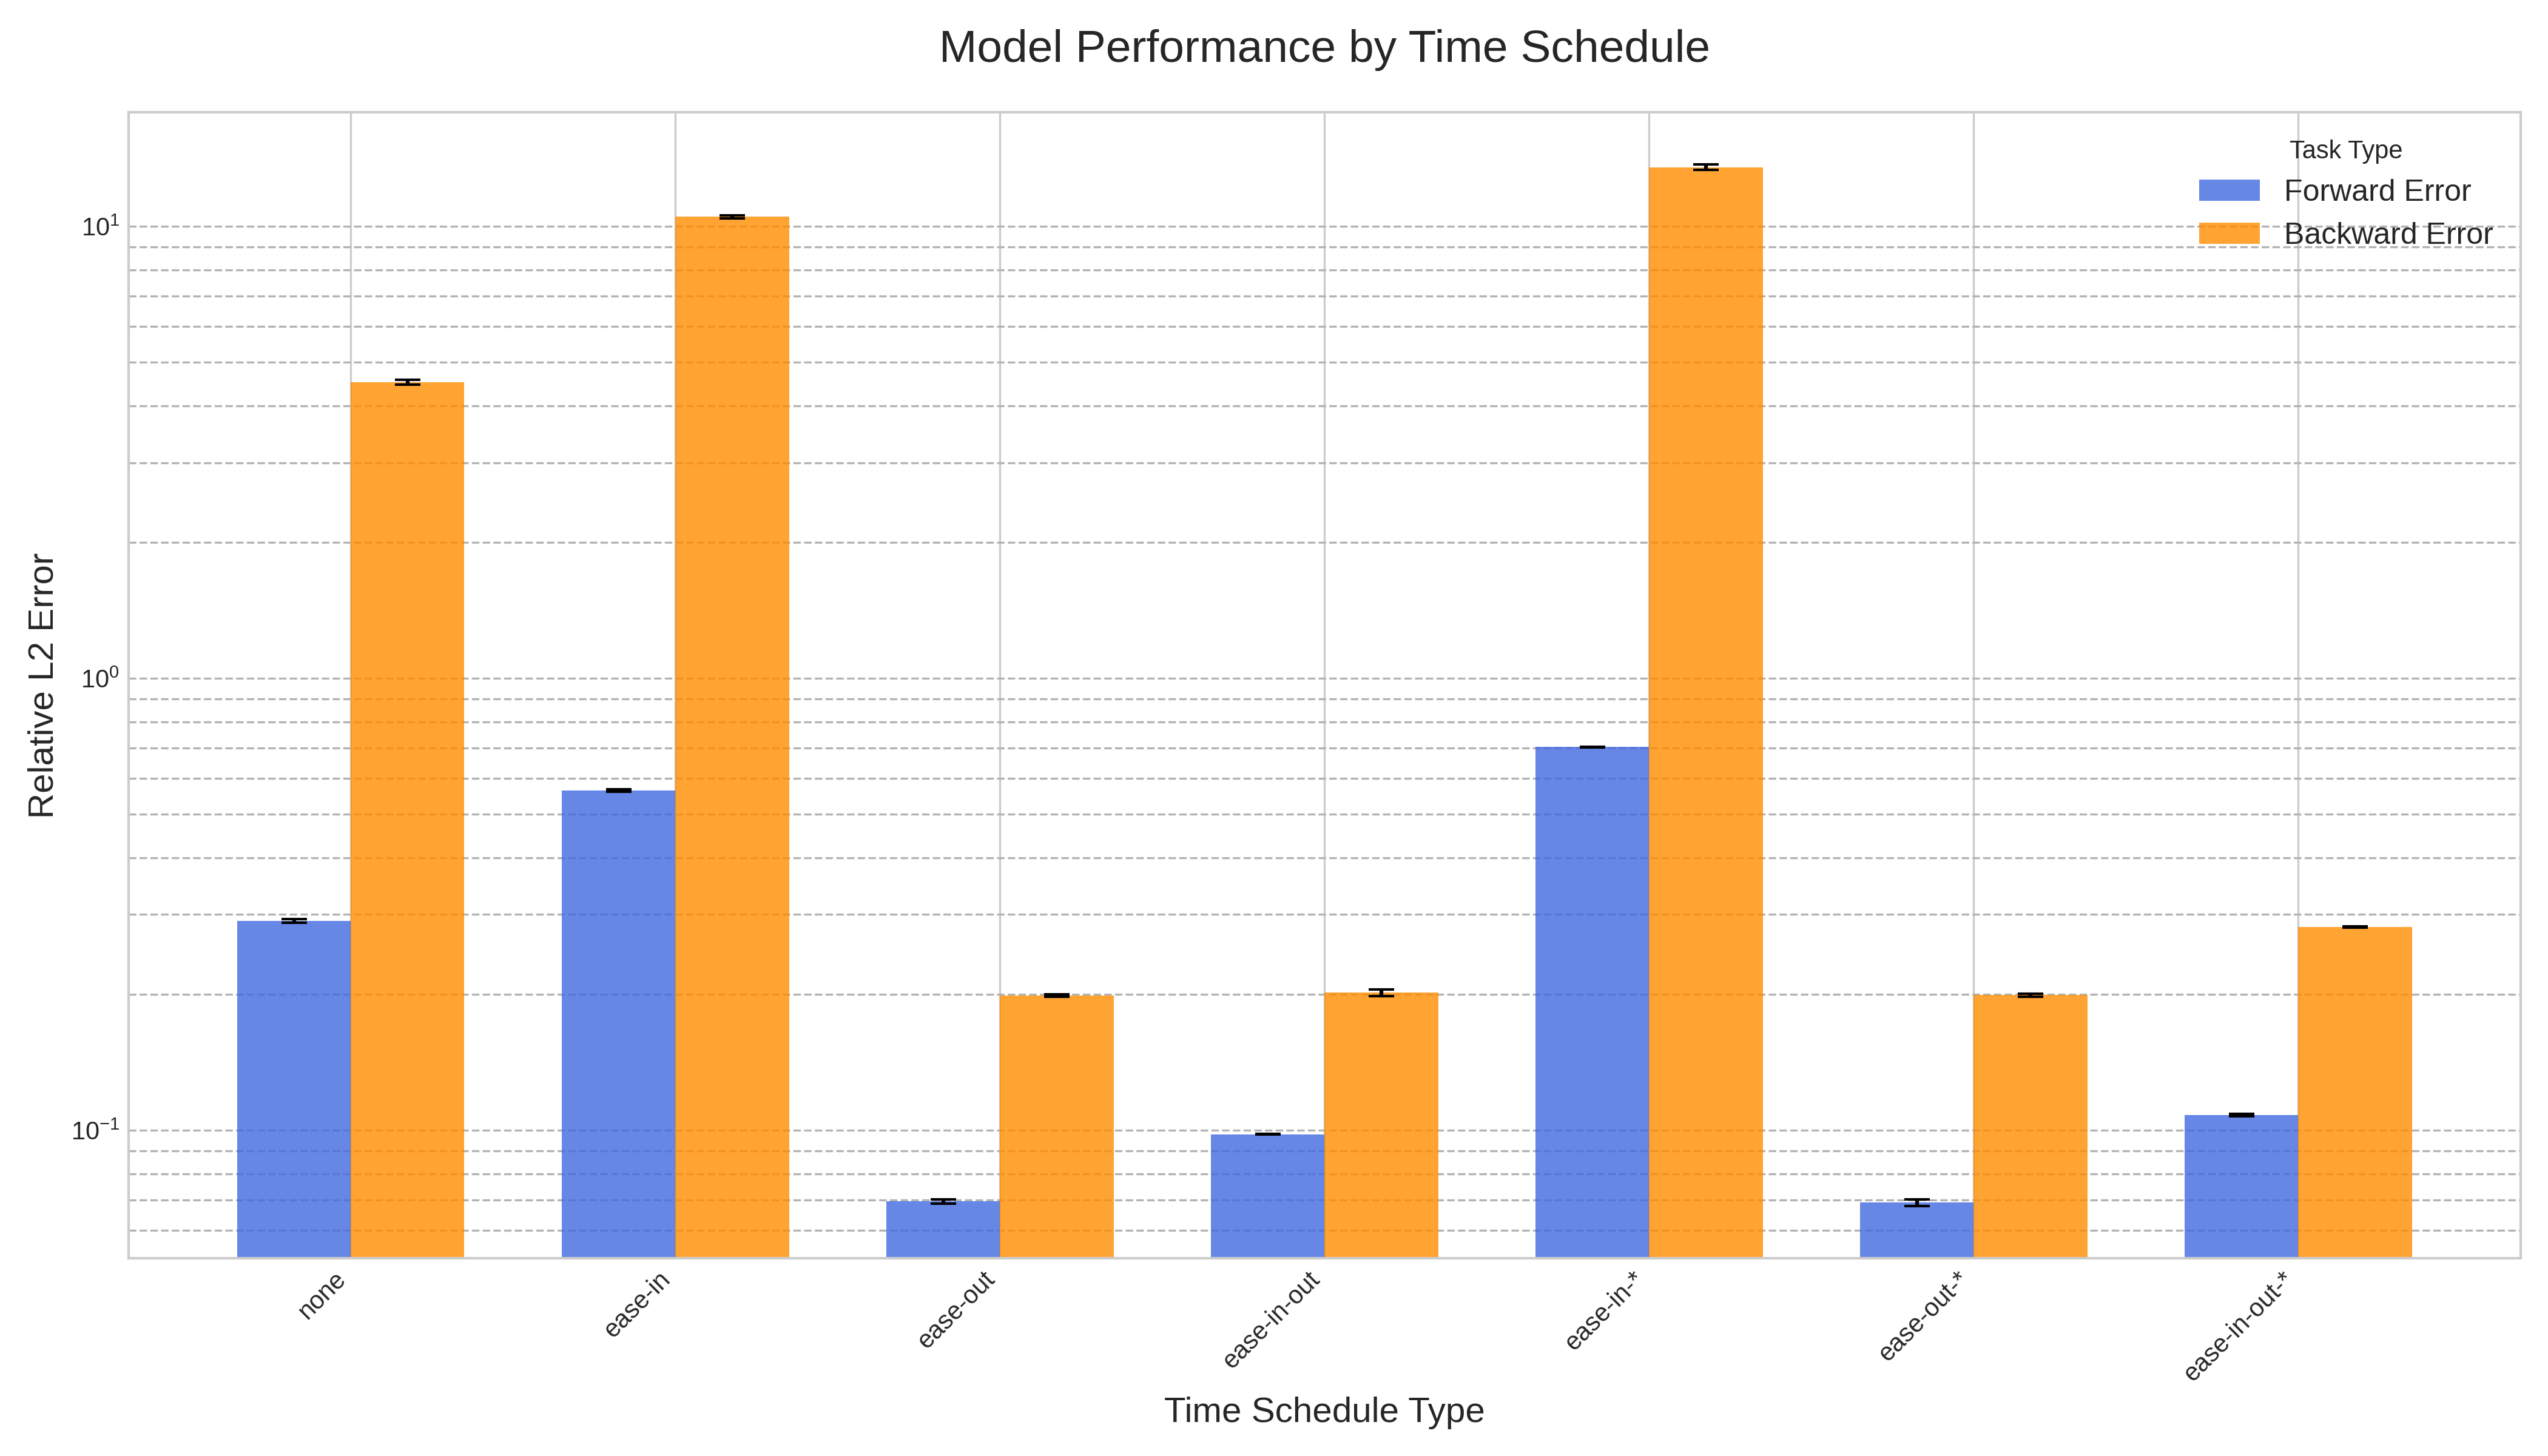
\includegraphics[width=\linewidth]{schedules.png}
\caption{Relative \(L^{2}\) error for forward and inverse tasks for each time change function \(\theta\)}\label{fig:schedulesr}
\end{figure}

Among the stable schedules, \texttt{ease-out} an \texttt{ease-out-*} achieve the best performance for both the forward and backward tasks. Interestingly, these schedules which only slow time down at \(t=1\) outperform those which also slow time down at \(t=0\). Furthermore, both \texttt{ease-out} and \texttt{ease-in-out} outperform their \texttt{-*} counterparts. This confirms our theory that in the case \(b = \frac{\varepsilon}{2}\), only condition (\ref{lem:thetaconditions:1}) of \Cref{lem:thetaconditions} is necessary and sufficient for a well-behaved time-changed drift.  Intuitively, an additional slowdown at \(t=0\) is misallocates the solver's finite computational budget to a non-problematic region of the time domain.

Indeed, the \texttt{ease-out} schedule is in a sense the \textit{minimal} time change schedule satisfying \Cref{lem:thetaconditions}:  it addresses the only singularity at \(t=1\) and its derivative decays linearly. Since our theory requires the derivative to decay \textit{at least} linearly, this schedule achieves condition (\ref{lem:thetaconditions:1}) without being overly smooth. The inferior performance of the \texttt{-*} variants, whose derivatives decay faster than any polynomial, suggests that this minimal approach is optimal and that excessive smoothness is not beneficial.

This analysis suggests that \textit{the time change should be a minimal intervention}, applied only to ensure numerical stability. Our results indicate that and there is no benefit to biasing the integration away from or towards any particular region of the generative path apart from to address the singularity at \(t=1\).

\paragraph{Non-uniform time sampling}
Having established \texttt{ease-out} as the optimal choice of \(\theta\), we investigate whether a non-uniform sampling of time \(t\) during training helps to improve performance. Intuitively, since a greater number of function evaluations of \(\widetilde{f}\) happen at times closer to \(1\) during sampling, these times should also be drawn more frequently during training to control approximation error. During training, we sample \(\tau \sim \operatorname{U}([0, 1])\) and assign \(t \leftarrow \theta(t)\). This is equivalent to sampling \(t\) as a random variable whose inverse CDF is \(\theta\) and whose corresponding PDF is \(\frac{1}{2\sqrt{1-t}}\) on \([0, 1]\).

% \subsection{Noise smoothness}
% We first experiment with

% Narrative for 1D goes as follows:
% \begin{enumerate}
%   \item to choose roughness of noise, look at graph of relative L2 error when projecting 1D dataset onto the RKHS of \(C\) for RBF kernel of different length scales
%   \item compare this to empirical results when training on differnet length scales
%   \item show experiment with time re-weightings and argue that the time change \(\theta(t) = t^{2}\) is best -- it outperforms even the ease-in-out schedule which we attribute to \textit{starvation} of the intermediate time steps
%   \item having establisehd \(\theta(t) = t^{2}\) as the best time change, show experiment where \(t\) is sampled according to \(u^{2}\) where \(u \sim \operatorname{U}[0, 1]\). This does not perform as well which we attribute to \textit{model starvation} -- not enough emphasis on crucial earlier time steps. hence we argue that the change-in-time is there primarily to mitigate the explosion in the coefficient on \(\eta\) and thus preventing amplification of training errors
%   \item compare with the "alternative parameterisation" where we only learn \(\mathop{\mathbb{E}}\qty[\xi_{1} \mid \xi_{0}, x_{t}]\) and show this does not work well
%   \item hence for the expensive 2D datasets we go ahead with uniform time sampling during training, and learn \(\varphi, \eta\)
% \end{enumerate}
\section{2D Dataset}\label{sec:darcy2}

% Narrative for 2D datasets goes as follows
% \begin{enumerate}
%   \item present results for different length scales
%   \item compare performance with FunDPS and vanilla stochatic interpolants baselines and show performance is very competitive with the former and (hopefully) far exceeds that of the latter
%   \item ablation: training the marginal model. performance not much worse, so it's useful in circumstances where we want to train less and are willing to give up some performance. likely due to diffusion paths being mainly driven by the conditioning on \(x_{t}\) not \(\xi_{0}\)
%   \item ablation: ODE. note that we can predict \(\xi_{1}\) given \(\xi_{0}\) using only one step. haven't yet done this experiment
% \end{enumerate}

% TODOs: dynamic sensors, sparse sensors
% TODOs: higher res inference for 2D